%\documentclass[12pt,letterpaper]{article}
\documentclass[12pt,a4paper]{article} % NEW

% packages
\usepackage[utf8]{inputenc}
\usepackage[T1]{fontenc}
\usepackage[margin=1in]{geometry} % ORIGINAL
\usepackage[skip=0.5cm]{parskip} % ORIGINAL
%\usepackage[skip=10pt plus1pt, indent=20pt]{parskip} % NEW
\usepackage{setspace}
\usepackage{amsmath}
\usepackage{times}
\usepackage{graphicx}
\usepackage{hyperref}
\usepackage[font=footnotesize]{caption}
\usepackage{relsize}
\usepackage{environ}
\usepackage[sorting=none]{biblatex}
\usepackage{tikz}
\usepackage{pgfplots}
\usepackage{paralist}
\usepackage{amssymb}
\usepackage{listings}
\usepackage{color}
\usepackage{titling}
\usepackage{blindtext}
\usepackage{titlesec}
\usepackage{subcaption}
\usepackage{multicol}
\usepackage{abstract}
\usepackage{float}
\usepackage{xcolor}
\usepackage[UKenglish]{uiomasterfp}
\usepackage{dirtree}

% --- stuff from google ---
% Add an extra layer of headers
\setcounter{secnumdepth}{4}

\titleformat{\paragraph}
{\normalfont\normalsize\bfseries}{\theparagraph}{1em}{}
\titlespacing*{\paragraph}
{0pt}{3.25ex plus 1ex minus .2ex}{1.5ex plus .2ex}

\edef\origparind{\the\parindent}
\usetikzlibrary{positioning}
\pgfplotsset{compat=1.16}
\parindent=\origparind\relax
\DeclareCaptionType{equ}[][]

\emergencystretch=1em

\makeatletter
\def\maketag@@@#1{\hbox{\m@th\normalfont\normalsize#1}}
\makeatother

% make text lines be further away from each other
%\setstretch{1.4}

\linespread{1.35} % ORIGINAL
%\linespread{1.3}
%\linespread{1.25}

% env for equations and mathematical expressions
\NewEnviron{EQUATIONS}{%
  \scalebox{1.25}{$\BODY$}
}

% set size and (something else?) for the section and subsection headers (I think)
%\titleformat*{\section}{\large\bfseries}
%\titleformat*{\subsection}{\normalsize\bfseries}

% make abstract header larger
\renewcommand{\abstractnamefont}{\normalfont\large\bfseries}

% make urls in references look way less unacceptable
\renewcommand{\UrlFont}{\small\rm}

\makeatletter
\newrobustcmd{\mkbiblege}[1]{%
  \begingroup
  \blx@blxinit
  \blx@setsfcodes
  <#1>
  \endgroup}
\makeatother

\DeclareFieldFormat{url}{\bibstring{url}\space\mkbiblege{\url{#1}}}
% --- stuff from google END ---

% --- lstlisting START ---
\definecolor{dkgreen}{rgb}{0,0.6,0}
\definecolor{gray}{rgb}{0.5,0.5,0.5}
\definecolor{mauve}{rgb}{0.58,0,0.82}
\definecolor{pycomment}{rgb}{.3,.3,.3}

\lstdefinestyle{cppcode}{
  frame=tb,
  aboveskip=3mm,
  belowskip=-0.8mm,
  showstringspaces=false,
  columns=flexible,
  basicstyle={\small\ttfamily},
  numbers=left,
  numberstyle=\tiny,
  keywordstyle=\color{blue},
  commentstyle=\color{dkgreen},
  stringstyle=\color{mauve},
  breaklines=true,
  breakatwhitespace=true,
  tabsize=3,
  morekeywords={int8_t, int16_t, int32_t, int64_t,
                uint8_t, uint16_t, uint32_t, uint64_t}
}

\lstdefinestyle{pycode}{
  frame=tb,
  framerule=.75pt,
  aboveskip=3mm,
  belowskip=-0.8mm,
  showstringspaces=false,
  columns=flexible,
  basicstyle={\small\ttfamily},
  numbers=left,
  numberstyle=\tiny,
  keywordstyle=\color{blue},
  commentstyle=\color{pycomment},
  stringstyle=\color{mauve},
  breaklines=true,
  breakatwhitespace=true,
  tabsize=3,
}

\lstdefinestyle{console}{
  frame=tb,
  framerule=.75pt,
  aboveskip=3mm,
  belowskip=-0.8mm,
  showstringspaces=false,
  columns=flexible,
  basicstyle={\small\ttfamily},
  keywordstyle=\color{blue},
  commentstyle=\color{pycomment},
  stringstyle=\color{mauve},
  breaklines=true,
  breakatwhitespace=true,
  tabsize=3,
}

\lstdefinestyle{pseudocode}{
  mathescape=true,
  frame=tb,
  aboveskip=3mm,
  belowskip=-0.8mm,
  showstringspaces=false,
  columns=flexible,
  basicstyle={\small\ttfamily},
  numbers=left,
  numberstyle=\tiny,
  keywordstyle=\color{black}\bfseries\em,
  breaklines=true,
  breakatwhitespace=true,
  tabsize=3,
  literate=
       {=}{$\leftarrow{}$}{1}
       {==}{$={}$}{1}
       {<=}{$\leq{}$}{1}
       {>=}{$\geq{}$}{1}
       {!=}{$\neq{}$}{1}
       {&&}{$\wedge{}$ }{1}
       {||}{$\vee{}$ }{1},
  morekeywords={else,begin,input,output,function,procedure,end,then,do,if,while,return,min,max}
}

\lstdefinestyle{vcf}{
  frame=tb,
  framerule=.75pt,
  language=,
  basicstyle={\small\ttfamily},
  breaklines=true,
}
% --- lstlisting END ---

\addbibresource{bibliography.bib}

\title{\textbf{Speeding up Genotyping through GPU Acceleration}}
\date{15th of May 2023}
\author{\Large{Master's Thesis}\\\\Jørgen Wictor Henriksen}

\begin{document}
% UiO front page
\uiomasterfp[author={Jørgen Wictor Henriksen},date={Spring 2023},dept={Department of Bioinformatics},color=blue,long,supervisors={Ivar Grytten \and Knut Rand \and Geir Kjetil Sandve},program={Programming and System Architecture},title={Speeding up Genotyping through GPU Acceleration},subtitle={}]

% title
%\maketitle
%\newpage

% abstract
\begin{abstract}
In the last few decades, high-throughput sequencing has steadily become more cost effective and accessible.
When sequencing a human genome today, it is not uncommon to produce hundreds of millions of short snippets of the genetic sequence.
These snippets are produced without knowledge of where they originate from in the original genome sequence or which bases in the snippet may be erroneous.
With the potential for millions of genomes being sequenced in the coming years, tools for analyzing the large amounts of genetic sequence data produced will become increasingly important.
Genotyping - the process of determining the genetic sequence variants present in the chromosomes of a genome - is a core application for such genetic sequence data.
Work in alignment-free genotyping, a new method that forgoes aligning each sequenced snippet to a reference genome sequence, have recently showed that statistical models on analysis of \textit{k}mers can yield competitive accuracies while being significantly faster compared to more traditional alignment-based methods.
A recently published genotyping tool, KAGE, showed that an alignment-free genotyper implemented in Python could yield competitive accuracies while being more than 10 times faster than any other known method.
This thesis explores how parts of KAGE that deal with large matrix- and array-operations can be GPU accelerated, and finally presents GKAGE, a GPU accelerated version of KAGE. 
GKAGE achieves up to 10 times speedup compared to KAGE and is able to genotype a human individual in only a few minutes on consumer grade hardware - significantly faster than any other known genotyping tool today.
\end{abstract}

\newpage

% table of contents
\tableofcontents
\newpage

% sections
\section{Introduction}
\blindtext

\newpage
\section{Background}

\subsection{Biology}

\subsubsection{DNA, Chromosomes and Genomes} \label{background:biology:dna_chromosomes_and_genomes}

DNA, or \textit{deoxyribonucleic acid}, is a type of molecule that contains all the genetic material found in the cells of all known living organisms \cite{nhgri_dna}. 
The molecule is composed of two complementary strands of \textit{nucleotides} that are twisted together to form a double helix structure, connected by bonds formed between complementary nucleotides.
The two strands are in turn composed of the four nucleotide bases: adenine (A), guanine (G), cytosine (C) and thymine (T), where A and T, and C and G are complementary bases \cite[p.15]{singh}.
Furthermore, the two complementary strands of nucleotide bases actually encode the precise same information.
This is because with knowledge of just one of the strands' nucleotide sequence, say \textit{strand$_1$}, we can determine the sequence of the other strand, \textit{strand$_2$}, by exchanging each nucleotide in \textit{strand$_1$} with their complements and finally reversing the strand to determine what \textit{strand$_2$}'s sequence is.

\begin{figure}[H]
\begin{center}
\scalebox{1}{
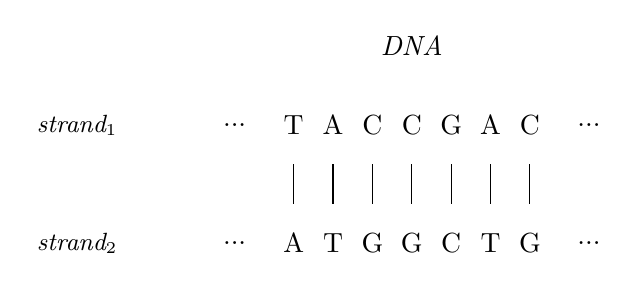
\begin{tikzpicture}
  % texts
  \node at(2.25,2.5)(title){\textit{DNA}};
  \node at(-2,0)(title){\small\textit{strand$_2$}};
  \node at(-2,1.5)(title){\small\textit{strand$_1$}};
  % lower nodes
  \node at(0,0)(n1){$...$};
  \node at(.75,0)(n2){A};
  \node at(1.25,0)(n3){T};
  \node at(1.75, 0)(n4){G};
  \node at(2.25,0)(n5){G};
  \node at(2.75,0)(n5){C};
  \node at(3.25,0)(n5){T};
  \node at(3.75,0)(n5){G};
  \node at(4.5,0)(n5){$...$};
  % upper nodes
  \node at(0,1.5)(n1){$...$};
  \node at(.75,1.5)(n2){T};
  \node at(1.25,1.5)(n3){A};
  \node at(1.75,1.5)(n4){C};
  \node at(2.25,1.5)(n5){C};
  \node at(2.75,1.5)(n5){G};
  \node at(3.25,1.5)(n5){A};
  \node at(3.75,1.5)(n5){C};
  \node at(4.5,1.5)(n5){$...$};
  % base pair bonds 
  \draw (.75,.5) -- (.75,1);
  \draw (1.25,.5) -- (1.25,1);
  \draw (1.75,.5) -- (1.75,1);
  \draw (2.25,.5) -- (2.25,1);
  \draw (2.75,.5) -- (2.75,1);
  \draw (3.25,.5) -- (3.25,1);
  \draw (3.75,.5) -- (3.75,1);
\end{tikzpicture}
}
\caption{A conceptual representation of a DNA molecule made up of two strands. The strands are composed of nucleotides forming base pairs where A (adenine) and T (thymine), and C (cytosine) and G (guanine) are complements of each other.}
\label{background:dna_and_chromosomes:figures:dna_strands}
\end{center}
\end{figure}

Relatively small differences in these DNA sequences are what differentiates individuals within the same species from one other.
It is therefore interesting to study these sequences of nucleotides encoding organisms' genetic information, as the encoded information can reveal details about both associated physical traits and diseases.
In human cells, these DNA strands are estimated to be roughly $3 * 10^{9}$ bases long \cite[p.13]{singh}.

DNA is organized into structures called \textit{chromosomes}. 
Humans have 23 chromosome pairs, making up a total of 46 chromosomes.
Each of the pairs include one version of the chromosome inherited from the male parent, and one version inherited from the female parent \cite{nhgri_chromosome}.

The term \textit{genome} can be used to refer to the complete genetic material of an organism.
In practice, however, the genome of an organism often simply refers to the complete DNA nucleotide sequence of one set of chromosomes for that organism \cite[p.13]{singh}.
Commonly in bioinformatics, one can also encounter the term \textit{reference genome}, referring to a theoretical reconstruction of an organism's genome created by scientists.
Such genome reconstructions are commonly used when examining new DNA sequences, often by aligning new DNA sequences to the reference in order to see at which positions their nucleotides differ and what differences are present at those positions \cite{gatk}.


\subsubsection{High-Throughput DNA sequencing}


\subsection{Nucleotide Binary Encoding} \label{background:nucleotide_binary_encoding}

DNA nucleotide sequences (described in section \ref{background:biology:dna_chromosomes_and_genomes}) inside computer software is commonly represented simply by a sequence of the 8 bit characters A, C, T and G (or alternatively the lowercase a, c, t and g).
This representation, however, is cumbersome to operate on and requires large amounts of memory to store.
To circumvent these issues, a widely adopted technique is to encode the nucleotides into binary form, often referred to as 2-bit encoding.
This leads to much quicker processing of nucleotide sequences and reduces the memory usage needed to store the sequences by 75\%.
This is achieved by realizing that only 2 bits, giving \textit{$2^2=4$} possible unique states, is enough to represent all of the four DNA nucleotides A, C, G and T.
The binary encoding can be extended further to represent whole nucleotide sequences in binary arrays.
For example, an integer array, if interpreted 2 consecutive bits at a time, can represent such a sequence.

\begin{figure}[H]
\begin{center}
\scalebox{1}{
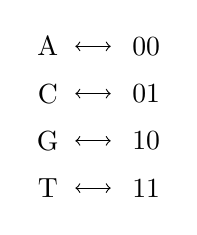
\begin{tikzpicture}
  \node at(0,0)(){T};
  \node at(0,.6)(){G};
  \node at(0,1.2)(){C};
  \node at(0,1.8)(){A};
  \node at(1.25,0)(){11};
  \node at(1.25,.6)(){10};
  \node at(1.25,1.2)(){01};
  \node at(1.25,1.8)(){00};
  \draw [<->](.35,0) -- (.8,0);
  \draw [<->](.35,.6) -- (.8,.6);
  \draw [<->](.35,1.2) -- (.8,1.2);
  \draw [<->](.35,1.8) -- (.8,1.8);
\end{tikzpicture}
}

\scalebox{1}{
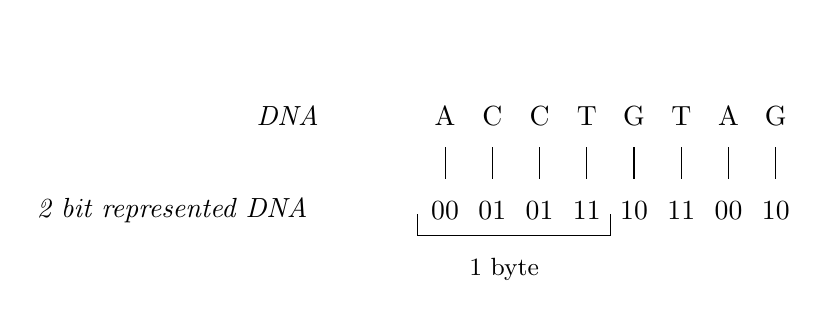
\begin{tikzpicture}
  \node at(0,1)(title){};
  \node at(-2,0)(){\textit{DNA}};
  \node at(-3.465,-1.2)(){\textit{2 bit represented DNA}};
  \node at(0,0)(){A};
  \node at(.6,0)(){C};
  \node at(1.2,0)(){C};
  \node at(1.8,0)(){T};
  \node at(2.4,0)(){G};
  \node at(3,0)(){T};
  \node at(3.6,0)(){A};
  \node at(4.2,0)(){G};
  \draw [](0,-.4) -- (0,-.8);
  \draw [](.6,-.4) -- (.6,-.8);
  \draw [](1.2,-.4) -- (1.2,-.8);
  \draw [](1.8,-.4) -- (1.8,-.8);
  \draw [](2.4,-.4) -- (2.4,-.8);
  \draw [](3,-.4) -- (3,-.8);
  \draw [](3.6,-.4) -- (3.6,-.8);
  \draw [](4.2,-.4) -- (4.2,-.8);
  \node at(0,-1.2)(){00};
  \node at(.6,-1.2)(){01};
  \node at(1.2,-1.2)(){01};
  \node at(1.8,-1.2)(){11};
  \node at(2.4,-1.2)(){10};
  \node at(3,-1.2)(){11};
  \node at(3.6,-1.2)(){00};
  \node at(4.2,-1.2)(){10};
  \draw [](-.35,-1.25) -- (-.35,-1.525);
  \draw [](2.1,-1.25) -- (2.1,-1.525);
  \draw [](-.35,-1.525) -- (2.1,-1.525);
  \node at(.75,-1.95)(){\small{1 byte}};
\end{tikzpicture}
}
\caption{A lookup table showing how nucleotides can be encoded using 2 bits and a DNA nucleotide sequence represented both as plain characters as well as its 2 bit encoded representation. Recall that computers use 8 bits to represent a single nucleotide with a character, whilst the 2 bit encoding only needs 2 bits to represent a nucleotide.}
\label{background:nucleotide_binary_encoding:figures:nucleotide_binary_encoding}
\end{center}
\end{figure}

\subsection{\textit{k}mers and the \textit{k}mer Counting Problem} \label{background:kmers_and_kmer_counting}
A \textit{k}mer is a substring of \textit{k} consecutive nucleotides that occur in a DNA (or RNA) sequence.
Because of how single nucleotides can be represented in a computer's memory using only 2 bits \ref{background:nucleotide_binary_encoding}, and how when we sequence an individual's genome we can not know which strand our sequenced read comes from, a popular choice of value for \textit{k} is 31 - the default value used in KAGE \ref{background:kage}.
The value 31 is used in KAGE for two reasons: 1) having an odd value for \textit{k} ensures that no \textit{k}mer is equal to its reverse complement, and 2) having \textit{k} equals 31 means we need $31*2=62$ bits to represent the \textit{k}mer in a computer's memory, thus the \textit{k}mer will fit inside a single 64-bit integer.

A common problem in various bioinformatics applications is to count the number of times each valid \textit{k}mer in a set of nucleotide sequences occurs in those sequences.
This problem is commonly referred to as \textit{k}mer counting.

\definecolor{kmer1}{RGB}{40,40,215}
\definecolor{kmer2}{RGB}{0,150,0}
\definecolor{kmer3}{RGB}{225,30,30}
\definecolor{kmer4}{RGB}{20,150,150}

\begin{figure}[H]
\begin{center}
\scalebox{1}{
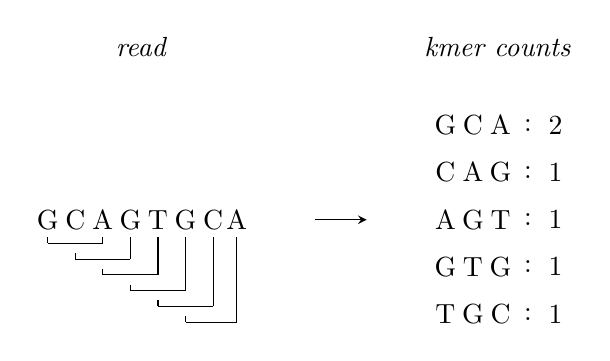
\begin{tikzpicture}
  % read
  \node at(1.2,2.2)(){\textit{read}};
  % sequence
  \node at(0,0){G};
  \node at(.35,0){C};
  \node at(.7,0){A};
  \node at(1.05,0){G};
  \node at(1.4,0){T};
  \node at(1.75,0){G};
  \node at(2.1,0){C};
  \node at(2.4,0){A};
  % kmer indicators
  % kmer 1
  \draw [](0,-.225) -- (0,-.3);
  \draw [](0,-.3) -- (.7,-.3);
  \draw [](.7,-.3) -- (.7,-.225);
  % kmer 2
  \draw [](.35,-.425) -- (.35,-.5);
  \draw [](.35,-.5) -- (1.05,-.5);
  \draw [](1.05,-.5) -- (1.05,-.225);
  % kmer 3
  \draw [](.7,-.625) -- (.7,-.7);
  \draw [](.7,-.7) -- (1.4,-.7);
  \draw [](1.4,-.7) -- (1.4,-.225);
  % kmer 4
  \draw [](1.05,-.825) -- (1.05,-.9);
  \draw [](1.05,-.9) -- (1.75,-.9);
  \draw [](1.75,-.9) -- (1.75,-.225);
  % kmer 5
  \draw [](1.4,-1.025) -- (1.4,-1.1);
  \draw [](1.4,-1.1) -- (2.1,-1.1);
  \draw [](2.1,-1.1) -- (2.1,-.225);
  % kmer 6
  \draw [](1.75,-1.225) -- (1.75,-1.3);
  \draw [](1.75,-1.3) -- (2.4,-1.3);
  \draw [](2.4,-1.3) -- (2.4,-.225);
  % arrow
  \draw [-stealth](3.4,0) -- (4.05,0);
  % k-mer counts
  \node at(5.725,2.2)(){\textit{kmer counts}};
  % kmer (count) representations
  % kmer 1
  \node at(5.05,1.2){G};
  \node at(5.4,1.2){C};
  \node at(5.75,1.2){A};
  \node at(6.1,1.2){:};
  \node at(6.45,1.2){2};
  % kmer 2
  \node at(5.05,.6){C};
  \node at(5.4,.6){A};
  \node at(5.75,.6){G};
  \node at(6.1,.6){:};
  \node at(6.45,.6){1};
  % kmer 3
  \node at(5.05,0){A};
  \node at(5.4,0){G};
  \node at(5.75,0){T};
  \node at(6.1,0){:};
  \node at(6.45,0){1};
  % kmer 4
  \node at(5.05,-.6){G};
  \node at(5.4,-.6){T};
  \node at(5.75,-.6){G};
  \node at(6.1,-.6){:};
  \node at(6.45,-.6){1};
  % kmer 5
  \node at(5.05,-1.2){T};
  \node at(5.4,-1.2){G};
  \node at(5.75,-1.2){C};
  \node at(6.1,-1.2){:};
  \node at(6.45,-1.2){1};
\end{tikzpicture}
}
\caption{
  \textit{Full} \textit{k}mer counting where we count the observed frequency of every valid \textit{k}mer in our read set.
}
\label{background:kmers_and_kmer_counting:full_kmer_counting:figure}
\end{center}
\end{figure}

The genotyping software tool KAGE, detailed in section \ref{background:kage}, contains \textit{k}mer counting as one of its core steps in its genotyping pipeline.
However, the \textit{k}mer counting process in KAGE is slightly different from the process commonly refered to by the term \textit{k}mer counting.
Rather than counting the observed frequency of every valid \textit{k}mer in a set of input reads, KAGE only counts the observed frequencies of every \textit{k}mer in a predefined set.
Given how many valid \textit{k}mers one can observe in a set of (hundreds of?) millions of reads (\textbf{cite?}), which is typical when sequencing and genotyping a human genome, not needing to store each of these with an associated count value makes this new \textit{k}mer counting variant significantly less memory and time consuming.

\begin{figure}[H]
\begin{center}
\scalebox{1}{
\begin{tikzpicture}
  % titles
  \node at(-0.55,3)(){\textit{input reads}};
  % read 1
  \node at(-1.85,2){G};
  \node at(-1.5,2){C};
  \node at(-1.15,2){\textcolor{kmer2}{A}};
  \node at(-.8,2){\textcolor{kmer2}{G}};
  \node at(-.45,2){\textcolor{kmer2}{T}};
  \node at(-.1,2){G};
  \node at(.25,2){C};
  \node at(.6,2){G};
  % read 2 
  \node at(-1.85,1.4){T};
  \node at(-1.5,1.4){C};
  \node at(-1.15,1.4){C};
  \node at(-.8,1.4){G};
  \node at(-.45,1.4){\textcolor{kmer3}{G}};
  \node at(-.1,1.4){\textcolor{kmer3}{T}};
  \node at(.25,1.4){\textcolor{kmer3}{C}};
  \node at(.6,1.4){T};
  % read 3 
  \node at(-1.85,.8){T};
  \node at(-1.5,.8){\textcolor{kmer2}{A}};
  \node at(-1.15,.8){\textcolor{kmer2}{G}};
  \node at(-.8,.8){\textcolor{kmer2}{T}};
  \node at(-.4,.8){T};
  \node at(-.1,.8){G};
  \node at(.25,.8){A};
  \node at(.6,.8){G};
  % read 4 
  \node at(-1.85,.2){C};
  \node at(-1.5,.2){\textcolor{kmer2}{A}};
  \node at(-1.15,.2){\textcolor{kmer2}{G}};
  \node at(-.8,.2){\textcolor{kmer2}{T}};
  \node at(-.4,.2){\textcolor{kmer4}{G}};
  \node at(-.1,.2){\textcolor{kmer4}{A}};
  \node at(.25,.2){\textcolor{kmer4}{C}};
  \node at(.6,.2){A};
  % read 5 
  \node at(-1.85,-.4){A};
  \node at(-1.5,-.4){\textcolor{kmer4}{G}};
  \node at(-1.15,-.4){\textcolor{kmer4}{A}};
  \node at(-.8,-.4){\textcolor{kmer4}{C}};
  \node at(-.4,-.4){C};
  \node at(-.1,-.4){\textcolor{kmer3}{G}};
  \node at(.25,-.4){\textcolor{kmer3}{T}};
  \node at(.6,-.4){\textcolor{kmer3}{C}};
  % Arrow
  \draw [-stealth](2.75,.8) -- (3.4,.8);
  % k-mer counts
  \node at(6.5,3)(){\textit{kmer counts}};
  % k-mer 1
  \node at(5.8,1.7){\textcolor{kmer1}{A}};
  \node at(6.15,1.7){\textcolor{kmer1}{T}};
  \node at(6.5,1.7){\textcolor{kmer1}{T}};
  \node at(6.85,1.7){:};
  \node at(7.2,1.7){0};
  % k-mer 2 
  \node at(5.8,1.1){\textcolor{kmer2}{A}};
  \node at(6.15,1.1){\textcolor{kmer2}{G}};
  \node at(6.5,1.1){\textcolor{kmer2}{T}};
  \node at(6.85,1.1){:};
  \node at(7.2,1.1){3};
  % k-mer 3 
  \node at(5.8,.5){\textcolor{kmer3}{G}};
  \node at(6.15,.5){\textcolor{kmer3}{T}};
  \node at(6.5,.5){\textcolor{kmer3}{C}};
  \node at(6.85,.5){:};
  \node at(7.2,.5){2};
  % k-mer 4 
  \node at(5.8,-.1){\textcolor{kmer4}{G}};
  \node at(6.15,-.1){\textcolor{kmer4}{A}};
  \node at(6.5,-.1){\textcolor{kmer4}{C}};
  \node at(6.85,-.1){:};
  \node at(7.2,-.1){2};
\end{tikzpicture}
}
\caption{
  \textit{Partial} \textit{k}mer counting where we only count the observed frequencies of \textit{k}mers present in a predefined set. In this example, our set of predefined \textit{k}mers is \{ATT, AGT, GTC, GAC\}. During counting, \textit{k}mers not present in this set are skipped.
}
\label{background:kmers_and_kmer_counting:partial_kmer_counting:figure}
\end{center}
\end{figure}

Henceforth in this thesis, we will in the favour of brevity refer to the former \textit{k}mer counting process where we count every valid \textit{k}mer's occurrence as \textit{full} \textit{k}mer counting, and to the latter process where we only count the occurrences of \textit{k}mers in a predefined set as \textit{partial} \textit{k}mer counting.

While several \textit{k}mer counting software tools have been developed in previous work, with at least one, Gerbil \cite{gerbil}, having support for GPU acceleration \cite{kmer_counting_tools}, these tools are designed to solve the \textit{full} \textit{k}mer counting problem.

\subsection{Graphical Processing Units} \label{background:graphical_processing_units}

\textit{Graphical Processing Units} (GPUs) are massively parallel processing units designed for high-throughput parallel computations.
This is as opposed to \textit{Central Processing Units} (CPUs), which are designed to quickly perform many serial computations.
GPUs were originally developed to accelerate computations performed on images, a highly parallel task where it is commonplace to have millions of relatively small independent computations that must be performed quickly in a single memory buffer.
Although GPUs have mainly been used for graphical computations, they have in recent years been adopted in other areas as well with the introduction of the \textit{General Purpose Graphical Processing Unit} (GPGPU) (\textbf{GPGPU cite}). 
The concept of the GPGPU is to use a GPU, which is designed for computer graphics, to perform computations in other domains where CPUs are typically used.
Fields such as artificial intelligence (\textbf{AI accelerated by GPU cite}) and the broader scientific computing have enjoyed great utility from GPUs, using them to accelerate embarassingly parallel problems, \textit{e}.\textit{g}., matrix operations.
Despite being similar in power consumption, a GPU can provide much higher instruction throughput and memory bandwidth compared to its CPU competitors.
These capability advantages exist in GPUs because they were specifically designed to perform well with regards to these dimensions.

As of 2023, Nvidia control the vast majority of the GPU market share, with only \textit{Advanced Micro Devices} (AMD) and Intel as current serious competitors (\textbf{try to find a serious cite}).
Furthermore, Nvidia GPUs with their CUDA programming model is considered to be the standard for scientific computing today (\textbf{cite}).
Although most of the GPUs manufactured by different GPU manufacturing companies are very similar in both architecture and compute models, the term \textit{GPU} will for the remainder of this thesis specifically refer to Nvidia GPUs, as the work presented in this thesis was developed and tested using only Nvidia GPUs.


\subsubsection{GPUs in Computers}

Two main computer GPU setups are prominent today: \textit{integrated} graphical processing units (iGPU) and \textit{discrete} graphical processing units (dGPU), with the latter being most common both for consumer desktop computers as well as for scientific computing cluster nodes.
iGPUs are GPUs integrated onto the same die as a computer's CPU, where the two share the same physical \textit{Random Access Memory} (RAM) unit.

\begin{figure}[h!]\label{figure:gpu-system}
\begin{center}
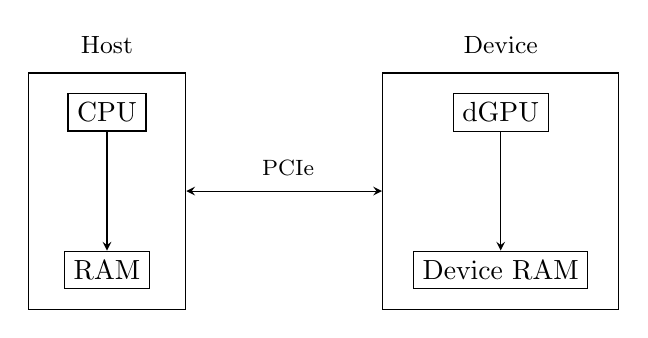
\begin{tikzpicture}

  \node at(0,2)[rectangle,draw](cpu){CPU};
  \node at(0,0)[rectangle,draw](cpuram){RAM};
  \node at(5,2)[rectangle,draw](gpu){dGPU};
  \node at(5,0)[rectangle,draw](gpuram){Device RAM};

  \node at(0,1)[rectangle,draw,minimum width=2cm,minimum height=3cm](host){};
  \node at(5,1)[rectangle,draw,minimum width=3cm,minimum height=3cm](device){};

  \draw [-stealth](cpu) -- (cpuram);
  \draw [-stealth](gpu) -- (gpuram);
  \draw [stealth-stealth](host) -- (device);

  \node at(2.3,1.3){\smaller PCIe};
  \node at(0,2.85){\small Host};
  \node at(5,2.85){\small Device};


\end{tikzpicture}
\caption{A typical CPU and dGPU setup.}
\end{center}
\end{figure}

\subsubsection{Programming Model and CUDA}

Modern GPUs can in effect be considered to be massive \textit{Single Instruction Multiple Data} (SIMD) machines. Strict flow control is therefore important; The same set of instructions should run in the same order for maximum utilization of the GPU's capability.
Furthermore, since GPUs are commonly a discrete compute unit from a computer's CPU, it contains its own \textit{Random Access Memory} (RAM) unit, requiring data to be copied from the ...


\subsection{Implementation Tools and Libraries} \label{background:implementation_tools_and_libraries}

This section will provide a brief introduction to some core programming languages and software libraries that were used in the work presented in this thesis.

\subsubsection{C and C++} \label{background:implementation_tools_and_libraries:c_and_cpp}
C and C++ are compiled general purpose programming languages.
C++ is a superset of C, and can in effect be considered to be C with classes among some other high-level functionality.
C and C++ are popular choices for implementing optimized and performant code.
They offer granular control over hardware and memory, where data such as arrays must be manually allocated and de-allocated.

\subsubsection{Python} \label{background:implementation_tools_and_libraries:python}
Python is an interpreted high-level general purpose programming language that has gained significant traction, including in the scientific computing community, in recent years \cite{python,python_popular}.
Since it is an interpreted language, Python in and of itself is not performant, and can in many instances be measured to be several orders of magnitude slower than similar implementations in performant compiled languages such as C and C++.
The Python interpreter is written in C, and thus, the Python programming language can naturally be extended with additional C and C++ code.
Because of its high-level and interpreted nature, it is well suited for quick software prototyping.
However, because of its ability to be extended with additional C and C++ code, many packages exist today that supplement Python with high-performance libraries, making Python a serious language candidate for scientific computing software today, albeit through calling upon optimized and performant C and C++ code.

\subsubsection{NumPy} \label{background:implementation_tools_and_libraries:numpy}
NumPy is a scientific computing library for Python that provides support for fast multi-dimensional arrays along with a multitude of mathematical and other types of functions to operate on arrays efficiently \cite{numpy}.
NumPy works as a Python interface to fast C and C++ code that implements the underlying functionalities.
This underlying code relies on vectorization and SIMD instructions to perform array operations fast. 
While NumPy's standard functionality is designed to run efficiently on a single CPU core, multithreading can be utilized to parallelize on the local data (SIMD), as well as the total work level (multithreading) at the same time.
Its flexible and easy-to-use interface along with its highly performant solutions that support a wide range of hardware have made it a popular choice for any array-based scientific computing in Python.


\subsubsection{CuPy} \label{background:implementation_tools_and_libraries:cupy}
CuPy is GPU accelerated NumPy \cite{numpy} and SciPy \cite{scipy} compatible array library that, much like NumPy \cite{numpy}, provides a multi-dimensional array object as well as mathematical functions and routines to operate on these arrays.
In fact, CuPy's interface is designed to closely follow that of NumPy, meaning that most array-based code written in NumPy can seamlessly be replaced with CuPy to GPU accelerate the array operations.
CuPy, unlike NumPy, will store array data in GPU memory, and all array routine and function calls made using CuPy arrays will be run on the GPU.

CuPy also offers some access to CUDA functionality such as CUDA streams used to copy memory to and from the GPU's memory while simultaneously processing data, and device synchronization to halt the CPU until a process started on the GPU has completed.
Additionally CuPy supports creating custom kernels that can operate on GPU allocated arrays, directly in Python.
These kernels are then JIT (just-in-time) compiled when the program first encounters the kernel.
Thus, CuPy provides a useful module where GPU accelerated implementations can be made directly with a NumPy-like array interface, also supporting more granular custom kernels that can operate on the data in these arrays directly inside Python.

\subsubsection{npstructures} \label{background:implementation_tools_and_libraries:npstructures}
npstructures (NumPy Structures) is a Python package built on top of NumPy that provides data structures with NumPy-like features to augment the NumPy library \cite{npstructures}.
This is achieved by building these new data structures using NumPy's underlying multi-dimensional array object and fast array routines.

Some of npstructures' data structures have been central in work done in this thesis.
Those data structures will therefore be detailed in this section.

\paragraph{Ragged Array}
A central feature in npstructures is its ragged array object, a two-dimensional array data structure with differing column lengths that provides NumPy-like behaviour and performance.
The ragged array object works as a drop in alternative to NumPy's multi-dimensional array object where one needs an array structure where the column lengths can vary, supporting many of the common NumPy functionalities such as multi-dimensional indexing, slicing, universal functions and a subset of the function interface.
\begin{figure}[H]
\begin{lstlisting}[language=Python,style=console]
>>> import numpy as np
>>> from npstructures import RaggedArray
>>> data = np.array([0, 1, 2, 3, 4, 5, 6, 7, 8])
>>> column_lengths = np.array([4, 2, 3])
>>> ra = RaggedArray(data, column_lengths)
>>> ra
ragged_array([0, 1, 2, 3]
[4, 5]
[6, 7, 8])
>>> ra.ravel()
array([0, 1, 2, 3, 4, 5, 6, 7, 8])
>>> type(ra.ravel())
<class 'numpy.ndarray'>
>>> np.sum(ra)
36
\end{lstlisting}
\caption{
  A simple illustration of how npstructures' data structures can be used directly in Python as drop-in augmentations to the NumPy library.
}
\label{background:implementation_tools_and_libraries:npstructures:figure:ragged_array_example}
\end{figure}

\paragraph{Hash Table and Counter}
npstructures also provides a memory efficient hash table built on top of the ragged array data structure.
This is designed to give dictionary-like behaviour for NumPy-arrays where chunks of key-value pairs can be operated on at once using fast NumPy array routines.
The hash table object is the base for a counter object that allows for counting of occurrences of a predefined set of keys.

The counter (built on top of the hash table) achieves its memory efficiency by implementing a type of bucketed hash table where a ragged array is used to represent the table. 
The number of rows of the array is equal to the number of buckets in the table, and the varying column lengths are equal to the bucket sizes.
Upon initialization, the hash table hashes every key in the static key-set provided and computes how many keys hash to each row in the ragged array, thereby determining the column lengths (bucket sizes) for each row.

\subsubsection{BioNumPy} \label{background:implementation_tools_and_libraries:bionumpy}
BioNumPy is a Python library built on top of NumPy that allows for easy and efficient representation and analysis of biological data \cite{bionumpy}.
This includes functionality for efficiently and correctly reading a multitude of different file types that are commonly used for storing biological data directly into NumPy arrays, fast encoding from character arrays representing biological sequences into 2-bit encoding for faster processing and better memory efficiency, and \textit{k}mer analysis support.

\subsubsection{pybind11} \label{background:implementation_tools_and_libraries:pybind11}
pybind11 \cite{pybind11} is a C++ library that provides easy-to-use macros and tools for creating bindings between Python and C++. 
Its main use case is to create Python bindings for existing C++ code.
Using pybind11, this can be achieved seamslessly by using C++ macros to expose C++ functions, classes and their methods to Python.
In addition, pybind11 also allows for direct use of certain Python types such as lists, tuples and dicts in C++, supporting both receiving and returning references to such Python objects in C++.
NumPy is also supported, making it easy to send NumPy array references to C++ functions where the C++ function is allowed the freedom to both read and write to the array's data.
While the work in this thesis evolves aroud GPU accelerating parts of a software tool written in Python, some of the solution implementations presented in this thesis were written partly in C++ for fast performance.
pybind11 were in these cases crucial in order to create the bindings from these C++ implementations, making them usable directly in Python.

\subsubsection{Snakemake} \label{background:snakemake}
Snakemake \cite{snakemake} is a workflow management system built on top of Python that allows for the creation of reproducible and scalable data analyses.
This is achieved through creating \textit{workflows}, using a human readable, Python based scripting language.
Such workflows are created as sets of rules, where each rule define how to produce one or more output files from one or more input files, for example by running a piece of software.
Once a workflow has been defined, Snakemake determines the order of which rules should be executed in order to produced the desired output.
Snakemake also ensures that workflows are reproducible by tracking input files, output files, and parameters used for executing rules, and parallelization of rule execution.



\subsection{KAGE} \label{background:kage}
KAGE \cite{kage} ...


\newpage
\section{Thesis Goal} \label{thesis_goal}

This thesis has two main goals.
One of the goals is to explore whether state-of-the-art genotyping can be sped up in any significant way by utilizing GPUs.
More specifically, this thesis will investigate whether alignment-free genotyping, which presently is significantly faster compared to alignment-based genotyping, can be sped up by utilizing the GPU.
In order to investigate this, we will attempt to integrate GPU accelerated functionality into a base alignment-free genotyper, KAGE, which is presently the fastest known genotyper that also yields competitive results.
The base genotyper, KAGE, is implemented in Python.
This leads to several possible avenues for integrating GPU support, either by low level implementations in C++ using CUDA or using existing Python packages providing GPU accelerated functionality.
This leads to the second goal of this thesis - to investigate and experiment with different ways of GPU accelerating existing Python code (that relies on array-programming libraries such as NumPy), and to discuss the advantages and drawbacks of using the different methods.
Finally, GPU accelerated functionality will be integrated into KAGE, resulting in GKAGE (GPU KAGE), and GKAGE will be benchmarked against KAGE to account for any potential speedup.


\newpage
\section{Methods} \label{methods}

In this section we describe how GPU acceleration support was provided for the KAGE genotyping pipeline, resulting in GKAGE - a version of KAGE where parts of the pipeline is GPU accelerated.

When developing GKAGE, we started with KAGE as a baseline and analysed the pipeline to find the most pronounced bottlenecks in terms of runtime.
We then examined whether these bottlenecks could benefit from GPU acceleration by taking into consideration the type of computations that were performed and whether they would be suitable for the GPU architecture as well as how much of the overall runtime the component constituted. 
We would then intuit whether the component in question would be worthwhile trying to GPU accelerate given the project's time constraints and estimated difficulty.

The baseline KAGE pipeline is split into two distinct processes: 1) counting the \textit{k}mer frequencies observed in the DNA reads of the individual being genotyped, and 2) genotyping the individual using a statistical model based on the observed and expected \textit{k}mer frequencies.
Initial benchmarking on a consumer desktop revealed that the \textit{k}mer counting step constituted more than 96\% of the total KAGE runtime, with \textit{k}mer counting taking 2080 seconds and the genotyping step taking 70 seconds for a total of 2150 seconds (35 minutes and 50 seconds) to genotype a full human genome.
Thus, the \textit{k}mer counting step, having such a clear margin for runtime improvement over the genotyping step, was the initial focus for GPU acceleration for potential runtime speedup.

\subsection{GPU Accelerating \textit{k}mer Counting}
While different GPU accelerated \textit{k}mer counting solutions such as Gerbil \cite{gerbil} have been developed in previous work, we opted to develop our own \textit{k}mer counting method because the \textit{k}mer counting problem solved in KAGE is slightly different than the typical \textit{k}mer counting problem described in section \ref{background:kmers_and_the_kmer_counting_problem}.
Rather than counting the frequency of every observed \textit{k}mer in the input reads, or even the frequency of every observed \textit{k}mer where the frequency is larger than some threshold, KAGE is only interested in counting the observed frequencies for a predetermined set of \textit{k}mers.
This revised problem is easier to solve in practice because the memory constraints are significantly less.
In the interest of brevity, we will refer to the typical \textit{k}mer counting problem described section \ref{background:kmers_and_the_kmer_counting_problem} as \textit{full kmer counting}, and the simpler problem where we only count the frequencies of a predetermined set of \textit{k}mers as \textit{partial kmer counting} \ref{methods:gpu_accelerating_kmer_counting:partial_kmer_counting}.

\definecolor{kmer1}{RGB}{40,40,215}
\definecolor{kmer2}{RGB}{0,150,0}
\definecolor{kmer3}{RGB}{225,30,30}
\definecolor{kmer4}{RGB}{20,150,150}

\begin{figure}[H]
\begin{center}
\scalebox{1}{
\begin{tikzpicture}
  % titles
  \node at(-0.55,3)(){\textit{input reads}};
  % read 1
  \node at(-1.85,2){G};
  \node at(-1.5,2){C};
  \node at(-1.15,2){\textcolor{kmer2}{A}};
  \node at(-.8,2){\textcolor{kmer2}{G}};
  \node at(-.45,2){\textcolor{kmer2}{T}};
  \node at(-.1,2){G};
  \node at(.25,2){C};
  \node at(.6,2){G};
  % read 2 
  \node at(-1.85,1.4){T};
  \node at(-1.5,1.4){C};
  \node at(-1.15,1.4){C};
  \node at(-.8,1.4){G};
  \node at(-.45,1.4){\textcolor{kmer3}{G}};
  \node at(-.1,1.4){\textcolor{kmer3}{T}};
  \node at(0.25,1.4){\textcolor{kmer3}{C}};
  \node at(.6,1.4){T};
  % read 3 
  \node at(-1.85,0.8){T};
  \node at(-1.5,0.8){\textcolor{kmer2}{A}};
  \node at(-1.15,0.8){\textcolor{kmer2}{G}};
  \node at(-.8,0.8){\textcolor{kmer2}{T}};
  \node at(-.4,0.8){T};
  \node at(-.1,0.8){G};
  \node at(.25,0.8){A};
  \node at(.6,0.8){G};
  % read 4 
  \node at(-1.85,0.2){C};
  \node at(-1.5,0.2){\textcolor{kmer2}{A}};
  \node at(-1.15,0.2){\textcolor{kmer2}{G}};
  \node at(-.8,0.2){\textcolor{kmer2}{T}};
  \node at(-.4,0.2){\textcolor{kmer4}{G}};
  \node at(-.1,0.2){\textcolor{kmer4}{A}};
  \node at(.25,0.2){\textcolor{kmer4}{C}};
  \node at(.6,0.2){A};
  % read 5 
  \node at(-1.85,-0.4){A};
  \node at(-1.5,-0.4){\textcolor{kmer4}{G}};
  \node at(-1.15,-0.4){\textcolor{kmer4}{A}};
  \node at(-.8,-0.4){\textcolor{kmer4}{C}};
  \node at(-.4,-0.4){C};
  \node at(-.1,-0.4){\textcolor{kmer3}{G}};
  \node at(.25,-0.4){\textcolor{kmer3}{T}};
  \node at(.6,-0.4){\textcolor{kmer3}{C}};
  % Arrow
  \draw [-stealth](2.75,1.25) -- (3.4,1.25);
  % k-mer counts
  \node at(6.5,3)(){\textit{kmer counts}};
  % k-mer 1
  \node at(5.8,2){\textcolor{kmer1}{A}};
  \node at(6.15,2){\textcolor{kmer1}{T}};
  \node at(6.5,2){\textcolor{kmer1}{T}};
  \node at(6.85,2){:};
  \node at(7.2,2){0};
  % k-mer 2 
  \node at(5.8,1.4){\textcolor{kmer2}{A}};
  \node at(6.15,1.4){\textcolor{kmer2}{G}};
  \node at(6.5,1.4){\textcolor{kmer2}{T}};
  \node at(6.85,1.4){:};
  \node at(7.2,1.4){3};
  % k-mer 3 
  \node at(5.8,0.8){\textcolor{kmer3}{G}};
  \node at(6.15,0.8){\textcolor{kmer3}{T}};
  \node at(6.5,0.8){\textcolor{kmer3}{C}};
  \node at(6.85,0.8){:};
  \node at(7.2,0.8){2};
  % k-mer 4 
  \node at(5.8,0.2){\textcolor{kmer4}{G}};
  \node at(6.15,0.2){\textcolor{kmer4}{A}};
  \node at(6.5,0.2){\textcolor{kmer4}{C}};
  \node at(6.85,0.2){:};
  \node at(7.2,0.2){2};
\end{tikzpicture}
}
\caption{
  In KAGE, we are only interested in counting the observed frequencies of a predefined set of \textit{k}mers, as opposed to every observed \textit{k}mer in the sequenced reads.
}
\label{methods:gpu_accelerating_kmer_counting:partial_kmer_counting}
\end{center}
\end{figure}


%In this section we describe how GPU acceleration support was provided for the KAGE genotyping pipeline, resulting in GKAGE - a version of KAGE where parts of the pipeline is GPU accelerated.

When developing GKAGE, we started with KAGE as a baseline and analysed the pipeline to find the most pronounced bottlenecks in terms of runtime.
We then examined whether these bottlenecks could benefit from GPU acceleration by taking into consideration the type of computations that were performed and whether they would be suitable for the GPU architecture as well as how much of the overall runtime the component constituted. 
We would then intuit whether the component in question would be worthwhile trying to GPU accelerate given the project's time constraints and estimated difficulty.

The baseline KAGE pipeline is split into two distinct processes: 1) counting the \textit{k}mer frequencies observed in the DNA reads of the individual being genotyped, and 2) genotyping the individual using a statistical model based on the observed and expected \textit{k}mer frequencies.
Initial benchmarking on a consumer desktop revealed that the \textit{k}mer counting step constituted more than 96\% of the total KAGE runtime, with \textit{k}mer counting taking 2080 seconds and the genotyping step taking 70 seconds for a total of 2150 seconds (35 minutes and 50 seconds) to genotype a full human genome.
Thus, the \textit{k}mer counting step, having such a clear margin for runtime improvement over the genotyping step, was the initial focus for GPU acceleration for potential runtime speedup.

%\subsection{GPU Support Directly in Python} \label{methods:gpu_support_directly_in_python}
...

%\subsection{Custom CUDA Implementations} \label{methods:custom_cuda_implementations}
...

%\subsection{Finding Bottleneck Components} \label{methods:finding_bottleneck_components}
...

%\subsection{Implementation Details}

\subsubsection{CUDA Hash Table for \textit{k}mer Counting}
In order to solve the \textit{k}mer counting problem described in section \ref{background:kmer_counting}, GKAGE uses a GPU accelerated static hash table.
%In order to solve the \textit{k}mer counting problem described in section \ref{background:kmer_counting}, GKAGE uses a GPU accelerated static hash table.
The hash table uses open addressing with a simple linear probing scheme for insertions (during initialization), counts and queries.
%In order to use the hash table for counting in Python, Python bindings are implemented using pybind11 \cite{pybind11} (Move this and add info about how this interplays with NumPy and CuPy arrays?). 

The hash table is implemented using Nvidia's CUDA framework (described in section \ref{background:graphical_processing_units:programming_model_and_cuda}. 
as a C++ class with two arrays, one for the keys and one for the values (counts), allocated in the GPU's global memory.
The class implements methods for the three main operations:
\begin{compactenum}
  \item
    Insertion: only once during initialization
  \item
    Counting: incrementing the values associated with each \textit{k}mer value in an array
  \item
    Querying: fetching the values associated with each \textit{k}mer value in an array, returning an array of the same size
\end{compactenum}

The methods accept arrays that are either allocated in the GPU's global memory or in the host RAM.
When calls are made with the latter, the class method will handle the allocation of GPU memory, copying of data between host and GPU, and de-allocation of GPU memory when the processing has completed.
In the case of queries where the input \textit{k}mers are located in the host RAM, the corresponding counts array will also be located in the host RAM.

All of the operations (insert, count and query) work on a single \textit{k}mer basis. 
Notably, all of the operations take in an array of \textit{k}mers, and all of the corresponding CUDA implementations launch a single thread for each \textit{k}mer to fulfill the operation that is supposed to happen for that \textit{k}mer.
For example, when counting \textit{k}mers, an array of \textit{n} \textit{k}mers will be provided, and \textit{n} CUDA threads will be started, each taking care of incrementing the count of a single \textit{k}mer in the hash table.

\begin{equation}
  p_0=hash(k) \bmod c \hspace{7em} p_{i}=(p_{i-1}+1) \bmod c
\end{equation}

\definecolor{misscolor}{RGB}{255,215,215}
\definecolor{hitcolor}{RGB}{215,255,215}
\definecolor{countcolor}{RGB}{240,240,240}

\begin{figure}[ht!]
\begin{center}
\scalebox{1}{
\begin{tikzpicture}

  \node at(-5.4,-7.59)(kmers){\textit{\smaller{in kmers}}};

  \node at(-4,-7.59)[draw,minimum width=0.65cm,minimum height=0.65cm](){\smaller{$k_0$}};
  \node at(-3.35,-7.59)[draw,minimum width=0.65cm,minimum height=0.65cm](){\smaller{$k_1$}};
  \node at(-2.7,-7.59)[draw,minimum width=0.65cm,minimum height=0.65cm](){\smaller{$k_2$}};
  \node at(-2.05,-7.59)[draw,minimum width=0.65cm,minimum height=0.65cm](){\smaller{$...$}};
  \node at(-1.4,-7.59)[draw,minimum width=0.65cm,minimum height=0.65cm](){\smaller{$k_n$}};

  \node at(-3.55,-0.6)[](thread){\smaller{\textit{single CUDA thread}}};
  \draw [](-2.7,-6.99) -- (-2.7,-1);
  \draw [-stealth](-2.7,-1) -- (-1,-1);

  \node at(1.15,-1)(hash){\smaller{\textit{$p_0=h=hash(k) \bmod c$}}};

  \draw [](3.325,-1) -- (5.7,-1);
  \draw [-stealth](5.7,-1) -- (5.7,-2.05);

  \node at(8.25,-1.5)[fill=misscolor,rounded corners](miss){\textit{\smaller{miss}}};

  \node at(3.185,-2.5)(indices){\textit{\smaller{indices}}};
  \node at(3.365,-3.35)(keys){\textit{\smaller{keys}}};
  \node at(3.2375,-4.2)(values){\textit{\smaller{values}}};

  \node at(4.4,-2.5)[minimum width=0.65cm,minimum height=0.65cm](){\smaller{$0$}};
  \node at(5.05,-2.5)[minimum width=0.65cm,minimum height=0.65cm](){\smaller{$1$}};
  \node at(5.7,-2.5)[minimum width=0.65cm,minimum height=0.65cm](){\smaller{$p_0$}};
  \node at(6.35,-2.5)[minimum width=0.65cm,minimum height=0.65cm](){\smaller{$3$}};
  \node at(7,-2.5)[minimum width=0.65cm,minimum height=0.65cm](){\smaller{$4$}};
  \node at(7.65,-2.5)[minimum width=0.65cm,minimum height=0.65cm](){\smaller{$5$}};
  \node at(8.3,-2.5)[minimum width=0.65cm,minimum height=0.65cm](){\smaller{$...$}};

  \node at(4.4,-3.35)[draw,minimum width=0.65cm,minimum height=0.65cm](){\smaller{$...$}};
  \node at(5.05,-3.35)[draw,minimum width=0.65cm,minimum height=0.65cm](){\smaller{$...$}};
  \node at(5.7,-3.35)[draw,minimum width=0.65cm,minimum height=0.65cm,fill=misscolor](){\smaller{$...$}};
  \node at(6.35,-3.35)[draw,minimum width=0.65cm,minimum height=0.65cm](){\smaller{$k$}};
  \node at(7,-3.35)[draw,minimum width=0.65cm,minimum height=0.65cm](){\smaller{$...$}};
  \node at(7.65,-3.35)[draw,minimum width=0.65cm,minimum height=0.65cm](){\smaller{$...$}};
  \node at(8.3,-3.35)[draw,minimum width=0.65cm,minimum height=0.65cm](){\smaller{$...$}};

  \node at(4.4,-4.2)[draw,minimum width=0.65cm,minimum height=0.65cm](){\smaller{$0$}};
  \node at(5.05,-4.2)[draw,minimum width=0.65cm,minimum height=0.65cm](){\smaller{$0$}};
  \node at(5.70,-4.2)[draw,minimum width=0.65cm,minimum height=0.65cm](){\smaller{$0$}};
  \node at(6.35,-4.2)[draw,minimum width=0.65cm,minimum height=0.65cm](){\smaller{$0$}};
  \node at(7,-4.2)[draw,minimum width=0.65cm,minimum height=0.65cm](){\smaller{$0$}};
  \node at(7.65,-4.2)[draw,minimum width=0.65cm,minimum height=0.65cm](){\smaller{$0$}};
  \node at(8.3,-4.2)[draw,minimum width=0.65cm,minimum height=0.65cm](){\smaller{$0$}};

  \draw [-stealth](5.7,-4.85) -- (5.7,-5.5);

  \node at(5.7,-6)(hash){\smaller{\textit{$p_1=h+1 \bmod c$}}};

  \draw [](5.7,-6.5) -- (5.7,-6.85);
  \draw [](5.7,-6.85) -- (6.35,-6.85);
  \draw [-stealth](6.35,-6.85) -- (6.35,-7.15);

  \node at(8.25,-6)[fill=hitcolor,rounded corners](hit){\textit{\smaller{hit}}};

  \node at(3.185,-7.59)(indices){\textit{\smaller{indices}}};
  \node at(3.365,-8.44)(keys){\textit{\smaller{keys}}};
  \node at(3.2375,-9.29)(values){\textit{\smaller{values}}};

  \node at(4.4,-7.59)[minimum width=0.65cm,minimum height=0.65cm](){\smaller{$0$}};
  \node at(5.05,-7.59)[minimum width=0.65cm,minimum height=0.65cm](){\smaller{$1$}};
  \node at(5.7,-7.59)[minimum width=0.65cm,minimum height=0.65cm](){\smaller{$2$}};
  \node at(6.35,-7.59)[minimum width=0.65cm,minimum height=0.65cm](){\smaller{$p_1$}};
  \node at(7,-7.59)[minimum width=0.65cm,minimum height=0.65cm](){\smaller{$4$}};
  \node at(7.65,-7.59)[minimum width=0.65cm,minimum height=0.65cm](){\smaller{$5$}};
  \node at(8.3,-7.59)[minimum width=0.65cm,minimum height=0.65cm](){\smaller{$...$}};

  \node at(4.4,-8.44)[draw,minimum width=0.65cm,minimum height=0.65cm](){\smaller{$...$}};
  \node at(5.05,-8.44)[draw,minimum width=0.65cm,minimum height=0.65cm](){\smaller{$...$}};
  \node at(5.7,-8.44)[draw,minimum width=0.65cm,minimum height=0.65cm](){\smaller{$...$}};
  \node at(6.35,-8.44)[draw,minimum width=0.65cm,minimum height=0.65cm,fill=hitcolor](){\smaller{$k$}};
  \node at(7,-8.44)[draw,minimum width=0.65cm,minimum height=0.65cm](){\smaller{$...$}};
  \node at(7.65,-8.44)[draw,minimum width=0.65cm,minimum height=0.65cm](){\smaller{$...$}};
  \node at(8.3,-8.44)[draw,minimum width=0.65cm,minimum height=0.65cm](){\smaller{$...$}};

  \node at(4.4,-9.29)[draw,minimum width=0.65cm,minimum height=0.65cm](){\smaller{$0$}};
  \node at(5.05,-9.29)[draw,minimum width=0.65cm,minimum height=0.65cm](){\smaller{$0$}};
  \node at(5.70,-9.29)[draw,minimum width=0.65cm,minimum height=0.65cm](){\smaller{$0$}};
  \node at(6.35,-9.29)[draw,minimum width=0.65cm,minimum height=0.65cm](){\smaller{$0$}};
  \node at(7,-9.29)[draw,minimum width=0.65cm,minimum height=0.65cm](){\smaller{$0$}};
  \node at(7.65,-9.29)[draw,minimum width=0.65cm,minimum height=0.65cm](){\smaller{$0$}};
  \node at(8.3,-9.29)[draw,minimum width=0.65cm,minimum height=0.65cm](){\smaller{$0$}};

  \draw [-stealth](6.35,-9.94) -- (6.35,-10.59);

  \node at(8.25,-10.265)[fill=countcolor,rounded corners](count){\textit{\smaller{count}}};

  \node at(3.185,-11.03)(indices){\textit{\smaller{indices}}};
  \node at(3.365,-11.88)(keys){\textit{\smaller{keys}}};
  \node at(3.2375,-12.73)(values){\textit{\smaller{values}}};

  \node at(4.4,-11.03)[minimum width=0.65cm,minimum height=0.65cm](){\smaller{$0$}};
  \node at(5.05,-11.03)[minimum width=0.65cm,minimum height=0.65cm](){\smaller{$1$}};
  \node at(5.7,-11.03)[minimum width=0.65cm,minimum height=0.65cm](){\smaller{$2$}};
  \node at(6.35,-11.03)[minimum width=0.65cm,minimum height=0.65cm](){\smaller{$p_1$}};
  \node at(7,-11.03)[minimum width=0.65cm,minimum height=0.65cm](){\smaller{$4$}};
  \node at(7.65,-11.03)[minimum width=0.65cm,minimum height=0.65cm](){\smaller{$5$}};
  \node at(8.3,-11.03)[minimum width=0.65cm,minimum height=0.65cm](){\smaller{$...$}};

  \node at(4.4,-11.88)[draw,minimum width=0.65cm,minimum height=0.65cm](){\smaller{$...$}};
  \node at(5.05,-11.88)[draw,minimum width=0.65cm,minimum height=0.65cm](){\smaller{$...$}};
  \node at(5.7,-11.88)[draw,minimum width=0.65cm,minimum height=0.65cm](){\smaller{$...$}};
  \node at(6.35,-11.88)[draw,minimum width=0.65cm,minimum height=0.65cm](){\smaller{$k$}};
  \node at(7,-11.88)[draw,minimum width=0.65cm,minimum height=0.65cm](){\smaller{$...$}};
  \node at(7.65,-11.88)[draw,minimum width=0.65cm,minimum height=0.65cm](){\smaller{$...$}};
  \node at(8.3,-11.88)[draw,minimum width=0.65cm,minimum height=0.65cm](){\smaller{$...$}};

  \node at(4.4,-12.73)[draw,minimum width=0.65cm,minimum height=0.65cm](){\smaller{$0$}};
  \node at(5.05,-12.73)[draw,minimum width=0.65cm,minimum height=0.65cm](){\smaller{$0$}};
  \node at(5.70,-12.73)[draw,minimum width=0.65cm,minimum height=0.65cm](){\smaller{$0$}};
  \node at(6.35,-12.73)[draw,minimum width=0.65cm,minimum height=0.65cm](){\smaller{$1$}};
  \node at(7,-12.73)[draw,minimum width=0.65cm,minimum height=0.65cm](){\smaller{$0$}};
  \node at(7.65,-12.73)[draw,minimum width=0.65cm,minimum height=0.65cm](){\smaller{$0$}};
  \node at(8.3,-12.73)[draw,minimum width=0.65cm,minimum height=0.65cm](){\smaller{$0$}};

  \draw [](4.075,-13.5) -- (8.625,-13.5);
  \draw [](4.075,-13.4) -- (4.075,-13.6);
  \draw [](8.625,-13.4) -- (8.625,-13.6);
  \node at(6.35,-13.85)(c){\smaller{\textit{c}}};

\end{tikzpicture}
}
\caption{As an array of 64-bit integer encoded kmers are counted by the hash table, each CUDA thread will compute the first probe position $p_0$ for each individual kmer, and then continue probing by linearly moving up to the next consecutive slot until either an empty slot or the original kmer handled by the thread is observed. If en empty slot is observed, the thread terminates. If the original kmer is observed, the value at the current slot is increased.}
\label{figure:cucounter_hashtable}
\end{center}
\end{figure}


%\subsection{CUDA Hash Table for \textit{k}mer Counting}
In order to solve the \textit{k}mer counting problem described in section ?, GKAGE uses a GPU accelerated static hash table.
%In order to solve the \textit{k}mer counting problem described in section \ref{background:kmer_counting}, GKAGE uses a GPU accelerated static hash table.
The hash table uses open addressing with a simple linear probing scheme for insertions (during initialization), counts and queries.

The CUDA hash table is implemented as a C++ class with two arrays, one for the keys and one for the values (counts), allocated in the GPU's global memory.
The class implements methods for the three main operations:
\begin{compactenum}
  \item
    Insertion: only once during initialization
  \item
    Counting: incrementing the values associated with each \textit{k}mer value in an array
  \item
    Querying: fetching the values associated with each \textit{k}mer value in an array, returning an array of the same size
\end{compactenum}

The methods accept arrays that are either allocated in the GPU's global memory or in the host RAM.
When calls are made with the latter, the class method will handle the allocation of GPU memory, copying of data between host and GPU, and de-allocation of GPU memory when the processing has completed.
In the case of queries where the input \textit{k}mers are located in the host RAM, the corresponding counts array will also be located in the host RAM.

In order to use the hash table for counting in Python, Python bindings are implemented using pybind11 \cite{pybind11}.

\definecolor{misscolor}{RGB}{255,215,215}
\definecolor{hitcolor}{RGB}{215,255,215}
\definecolor{countcolor}{RGB}{240,240,240}

\begin{figure}[ht!]
\begin{center}
\scalebox{1}{
\begin{tikzpicture}

  \node at(-5.4,-7.59)(kmers){\textit{\smaller{in kmers}}};

  \node at(-4,-7.59)[draw,minimum width=0.65cm,minimum height=0.65cm](){\smaller{$k_0$}};
  \node at(-3.35,-7.59)[draw,minimum width=0.65cm,minimum height=0.65cm](){\smaller{$k_1$}};
  \node at(-2.7,-7.59)[draw,minimum width=0.65cm,minimum height=0.65cm](){\smaller{$k_2$}};
  \node at(-2.05,-7.59)[draw,minimum width=0.65cm,minimum height=0.65cm](){\smaller{$...$}};
  \node at(-1.4,-7.59)[draw,minimum width=0.65cm,minimum height=0.65cm](){\smaller{$k_n$}};

  \node at(-3.55,-0.6)[](thread){\smaller{\textit{single CUDA thread}}};
  \draw [](-2.7,-6.99) -- (-2.7,-1);
  \draw [-stealth](-2.7,-1) -- (-1,-1);

  \node at(1.15,-1)(hash){\smaller{\textit{$p_0=h=hash(k) \bmod c$}}};

  \draw [](3.325,-1) -- (5.7,-1);
  \draw [-stealth](5.7,-1) -- (5.7,-2.05);

  \node at(8.25,-1.5)[fill=misscolor,rounded corners](miss){\textit{\smaller{miss}}};

  \node at(3.185,-2.5)(indices){\textit{\smaller{indices}}};
  \node at(3.365,-3.35)(keys){\textit{\smaller{keys}}};
  \node at(3.2375,-4.2)(values){\textit{\smaller{values}}};

  \node at(4.4,-2.5)[minimum width=0.65cm,minimum height=0.65cm](){\smaller{$0$}};
  \node at(5.05,-2.5)[minimum width=0.65cm,minimum height=0.65cm](){\smaller{$1$}};
  \node at(5.7,-2.5)[minimum width=0.65cm,minimum height=0.65cm](){\smaller{$p_0$}};
  \node at(6.35,-2.5)[minimum width=0.65cm,minimum height=0.65cm](){\smaller{$3$}};
  \node at(7,-2.5)[minimum width=0.65cm,minimum height=0.65cm](){\smaller{$4$}};
  \node at(7.65,-2.5)[minimum width=0.65cm,minimum height=0.65cm](){\smaller{$5$}};
  \node at(8.3,-2.5)[minimum width=0.65cm,minimum height=0.65cm](){\smaller{$...$}};

  \node at(4.4,-3.35)[draw,minimum width=0.65cm,minimum height=0.65cm](){\smaller{$...$}};
  \node at(5.05,-3.35)[draw,minimum width=0.65cm,minimum height=0.65cm](){\smaller{$...$}};
  \node at(5.7,-3.35)[draw,minimum width=0.65cm,minimum height=0.65cm,fill=misscolor](){\smaller{$...$}};
  \node at(6.35,-3.35)[draw,minimum width=0.65cm,minimum height=0.65cm](){\smaller{$k$}};
  \node at(7,-3.35)[draw,minimum width=0.65cm,minimum height=0.65cm](){\smaller{$...$}};
  \node at(7.65,-3.35)[draw,minimum width=0.65cm,minimum height=0.65cm](){\smaller{$...$}};
  \node at(8.3,-3.35)[draw,minimum width=0.65cm,minimum height=0.65cm](){\smaller{$...$}};

  \node at(4.4,-4.2)[draw,minimum width=0.65cm,minimum height=0.65cm](){\smaller{$0$}};
  \node at(5.05,-4.2)[draw,minimum width=0.65cm,minimum height=0.65cm](){\smaller{$0$}};
  \node at(5.70,-4.2)[draw,minimum width=0.65cm,minimum height=0.65cm](){\smaller{$0$}};
  \node at(6.35,-4.2)[draw,minimum width=0.65cm,minimum height=0.65cm](){\smaller{$0$}};
  \node at(7,-4.2)[draw,minimum width=0.65cm,minimum height=0.65cm](){\smaller{$0$}};
  \node at(7.65,-4.2)[draw,minimum width=0.65cm,minimum height=0.65cm](){\smaller{$0$}};
  \node at(8.3,-4.2)[draw,minimum width=0.65cm,minimum height=0.65cm](){\smaller{$0$}};

  \draw [-stealth](5.7,-4.85) -- (5.7,-5.5);

  \node at(5.7,-6)(hash){\smaller{\textit{$p_1=h+1 \bmod c$}}};

  \draw [](5.7,-6.5) -- (5.7,-6.85);
  \draw [](5.7,-6.85) -- (6.35,-6.85);
  \draw [-stealth](6.35,-6.85) -- (6.35,-7.15);

  \node at(8.25,-6)[fill=hitcolor,rounded corners](hit){\textit{\smaller{hit}}};

  \node at(3.185,-7.59)(indices){\textit{\smaller{indices}}};
  \node at(3.365,-8.44)(keys){\textit{\smaller{keys}}};
  \node at(3.2375,-9.29)(values){\textit{\smaller{values}}};

  \node at(4.4,-7.59)[minimum width=0.65cm,minimum height=0.65cm](){\smaller{$0$}};
  \node at(5.05,-7.59)[minimum width=0.65cm,minimum height=0.65cm](){\smaller{$1$}};
  \node at(5.7,-7.59)[minimum width=0.65cm,minimum height=0.65cm](){\smaller{$2$}};
  \node at(6.35,-7.59)[minimum width=0.65cm,minimum height=0.65cm](){\smaller{$p_1$}};
  \node at(7,-7.59)[minimum width=0.65cm,minimum height=0.65cm](){\smaller{$4$}};
  \node at(7.65,-7.59)[minimum width=0.65cm,minimum height=0.65cm](){\smaller{$5$}};
  \node at(8.3,-7.59)[minimum width=0.65cm,minimum height=0.65cm](){\smaller{$...$}};

  \node at(4.4,-8.44)[draw,minimum width=0.65cm,minimum height=0.65cm](){\smaller{$...$}};
  \node at(5.05,-8.44)[draw,minimum width=0.65cm,minimum height=0.65cm](){\smaller{$...$}};
  \node at(5.7,-8.44)[draw,minimum width=0.65cm,minimum height=0.65cm](){\smaller{$...$}};
  \node at(6.35,-8.44)[draw,minimum width=0.65cm,minimum height=0.65cm,fill=hitcolor](){\smaller{$k$}};
  \node at(7,-8.44)[draw,minimum width=0.65cm,minimum height=0.65cm](){\smaller{$...$}};
  \node at(7.65,-8.44)[draw,minimum width=0.65cm,minimum height=0.65cm](){\smaller{$...$}};
  \node at(8.3,-8.44)[draw,minimum width=0.65cm,minimum height=0.65cm](){\smaller{$...$}};

  \node at(4.4,-9.29)[draw,minimum width=0.65cm,minimum height=0.65cm](){\smaller{$0$}};
  \node at(5.05,-9.29)[draw,minimum width=0.65cm,minimum height=0.65cm](){\smaller{$0$}};
  \node at(5.70,-9.29)[draw,minimum width=0.65cm,minimum height=0.65cm](){\smaller{$0$}};
  \node at(6.35,-9.29)[draw,minimum width=0.65cm,minimum height=0.65cm](){\smaller{$0$}};
  \node at(7,-9.29)[draw,minimum width=0.65cm,minimum height=0.65cm](){\smaller{$0$}};
  \node at(7.65,-9.29)[draw,minimum width=0.65cm,minimum height=0.65cm](){\smaller{$0$}};
  \node at(8.3,-9.29)[draw,minimum width=0.65cm,minimum height=0.65cm](){\smaller{$0$}};

  \draw [-stealth](6.35,-9.94) -- (6.35,-10.59);

  \node at(8.25,-10.265)[fill=countcolor,rounded corners](count){\textit{\smaller{count}}};

  \node at(3.185,-11.03)(indices){\textit{\smaller{indices}}};
  \node at(3.365,-11.88)(keys){\textit{\smaller{keys}}};
  \node at(3.2375,-12.73)(values){\textit{\smaller{values}}};

  \node at(4.4,-11.03)[minimum width=0.65cm,minimum height=0.65cm](){\smaller{$0$}};
  \node at(5.05,-11.03)[minimum width=0.65cm,minimum height=0.65cm](){\smaller{$1$}};
  \node at(5.7,-11.03)[minimum width=0.65cm,minimum height=0.65cm](){\smaller{$2$}};
  \node at(6.35,-11.03)[minimum width=0.65cm,minimum height=0.65cm](){\smaller{$p_1$}};
  \node at(7,-11.03)[minimum width=0.65cm,minimum height=0.65cm](){\smaller{$4$}};
  \node at(7.65,-11.03)[minimum width=0.65cm,minimum height=0.65cm](){\smaller{$5$}};
  \node at(8.3,-11.03)[minimum width=0.65cm,minimum height=0.65cm](){\smaller{$...$}};

  \node at(4.4,-11.88)[draw,minimum width=0.65cm,minimum height=0.65cm](){\smaller{$...$}};
  \node at(5.05,-11.88)[draw,minimum width=0.65cm,minimum height=0.65cm](){\smaller{$...$}};
  \node at(5.7,-11.88)[draw,minimum width=0.65cm,minimum height=0.65cm](){\smaller{$...$}};
  \node at(6.35,-11.88)[draw,minimum width=0.65cm,minimum height=0.65cm](){\smaller{$k$}};
  \node at(7,-11.88)[draw,minimum width=0.65cm,minimum height=0.65cm](){\smaller{$...$}};
  \node at(7.65,-11.88)[draw,minimum width=0.65cm,minimum height=0.65cm](){\smaller{$...$}};
  \node at(8.3,-11.88)[draw,minimum width=0.65cm,minimum height=0.65cm](){\smaller{$...$}};

  \node at(4.4,-12.73)[draw,minimum width=0.65cm,minimum height=0.65cm](){\smaller{$0$}};
  \node at(5.05,-12.73)[draw,minimum width=0.65cm,minimum height=0.65cm](){\smaller{$0$}};
  \node at(5.70,-12.73)[draw,minimum width=0.65cm,minimum height=0.65cm](){\smaller{$0$}};
  \node at(6.35,-12.73)[draw,minimum width=0.65cm,minimum height=0.65cm](){\smaller{$1$}};
  \node at(7,-12.73)[draw,minimum width=0.65cm,minimum height=0.65cm](){\smaller{$0$}};
  \node at(7.65,-12.73)[draw,minimum width=0.65cm,minimum height=0.65cm](){\smaller{$0$}};
  \node at(8.3,-12.73)[draw,minimum width=0.65cm,minimum height=0.65cm](){\smaller{$0$}};

  \draw [](4.075,-13.5) -- (8.625,-13.5);
  \draw [](4.075,-13.4) -- (4.075,-13.6);
  \draw [](8.625,-13.4) -- (8.625,-13.6);
  \node at(6.35,-13.85)(c){\smaller{\textit{c}}};

\end{tikzpicture}
}
\caption{As an array of 64-bit integer encoded kmers are counted by the hash table, each CUDA thread will compute the first probe position $p_0$ for each individual kmer, and then continue probing by linearly moving up to the next consecutive slot until either an empty slot or the original kmer handled by the thread is observed. If en empty slot is observed, the thread terminates. If the original kmer is observed, the value at the current slot is increased.}
\label{figure:cucounter_hashtable}
\end{center}
\end{figure}


\newpage
\section{Results} \label{results}

The following section will describe the results yielded from this master's project.

All benchmarking results presented in this chapter were determined by running the associated pieces of software on the following set of computers and then comparing the results.

\begin{center}
  \begin{tabular}{lll}
    \hline
      System                    & CPU                  & GPU                           \\
    \hline
      High-end compute server   & AMD EPYC 7742        & NVIDIA Tesla V100  (32GB)     \\
      Consumer desktop computer & Intel Core i5-11400F & NVIDIA GTX 1660 SUPER (6GB)   \\
    \hline
  \end{tabular}
\end{center}

\subsection{\textit{K}mer parsing from raw reads}
% make more precise reference to where GPU support for bionumpy is described
In section () I described how I implemented GPU support for parts of BioNumPy \cite{bionumpy} in order to allow for GPU acceleration when when parsing \textit{k}mers from raw reads in FASTA files.
In short: BioNumPy reads and parses chunks of \textit{k}mers from FASTA files by 
1) reading a chunk of raw bytes from the FASTA file, 
2) converting each DNA nucleotide found in the raw read data into 2-bit encoded representations (\ref{background:nucleotide_binary_encoding}), 
and 3) parsing all valid \textit{k}mers of the desired size from the 2-bit encoded reads data.

After copying the raw bytes read from the FASTA file directly to the GPU, steps 2) and 3) could be performed significantly faster on the GPU for large enough chunk sizes.

\subsection{\textit{K}mer counting}


\subsection{GKAGE vs KAGE} \label{results:gkage_vs_kage}

\begin{table}[H]
\begin{tabular}{lllll}
\cline{1-4}
\multicolumn{1}{|l|}{System} & \multicolumn{1}{l|}{Description}               & \multicolumn{1}{l|}{CPU}                  & \multicolumn{1}{l|}{GPU}                   &  \\ \cline{1-4}
\multicolumn{1}{|l|}{1}      & \multicolumn{1}{l|}{High-end compute server}   & \multicolumn{1}{l|}{AMD EPYC 7742}        & \multicolumn{1}{l|}{Nvidia Tesla V100}     &  \\ \cline{1-4}
\multicolumn{1}{|l|}{2}      & \multicolumn{1}{l|}{Consumer desktop} & \multicolumn{1}{l|}{Intel Core i5-11400F} & \multicolumn{1}{l|}{Nvidia GTX 1660 SUPER} &  \\ \cline{1-4}
\end{tabular}
\caption{
  The two systems used to benchmark GKAGE against KAGE to account for the speedup achieved through GPU acceleration.
  \textbf{System 1} is a high-end compute server with top-of-the-line hardware.
  \textbf{System 2} is a consumer grade desktop gaming computer.
}
\label{results:gkage_vs_kage:tables:systems}
\end{table}


\newpage
\section{Discussions} \label{discussions}

\subsection{Advantages and Drawbacks of Methods} \label{discussion:advantages_and_drawbacks_of_methods}
In section \ref{methods} we explored three different methods for GPU accelerating existing Python code.
Each of the methods we explored has a unique set of advantages and drawbacks.
The discipline of designing and implementing GPU programs is quite distinct from the more mainstream discipline of implementing programs meant to run serially on the CPU.
Becoming an expert GPU programmer can in many instances take years with all the technologies and tools available today.
Thus, an interesting dimension when assessing the advantages and drawbacks of the GPU acceleration methods we have explored is how seamless it is to implement the solution, particularly for someone with little or no experience in GPU programming.
%Other metrics we will discuss include how seamless the integration of a solution into Python is, how quickly a solution can be implemented compared to the alternative methods, among other per-method details.
We will additionally consider how seamless integration into Python is, and of course, the potential for performance.

\subsubsection{Using CuPy as a NumPy Drop-in Replacement} \label{discussion:using_cupy_as_a_numpy_drop_in_replacement}
The first GPU acceleration method we explored in section \ref{methods:preliminary_testing}, was to use CuPy, a GPU accelerated array library with an interface designed to closely follow NumPy, as a drop-in replacement for NumPy. 

\paragraph{Advantages}
This method is ideal in cases where an already existing Python solution based on NumPy exists.
Depending on the complexity of the program architecture, replacing the NumPy module with CuPy can yield seamless and immediate GPU acceleration without the need to implement any GPU functionality, understand the GPU hardware or leave the Python ecosystem.
This technique is in such instances, by a large margin, the fastest way of implementing GPU acceleration.
In cases where no existing solution exists to transform, CuPy is still an adequate tool for "quick and dirty" testing with seamless GPU acceleration directly in Python.
Additionally, this method does not require deep knowledge or understanding of the GPU hardware and architecture, as the routines and functions are implemented by the CuPy developers.
That being said, some knowledge about GPUs may still be helpful, as it can guide decision making about what type of NumPy code may best be suited for GPU acceleration and how the data flow may be best optimized.

\paragraph{Drawbacks}
While an advantage of CuPy is that it allows for seamless "quick and dirty" testing directly in Python, this conversely also introduces a drawback of this method.
Many solutions implemented using NumPy are designed for fast processing on the CPU.
While such solutions may seem like good candidates for GPU acceleration, this match is not guaranteed.
Additionally, because NumPy and CuPy are Python libraries, they suffer from many unnecessary data allocations and copies when nested Python expressions with arrays are computed.
An example highlighting this issue is the log of the probability mass function (LOGPMF) described in section \ref{methods:gpu_accelerating_genotyping}.
As the nested LOGPMF expression is computed using CuPy arrays, Python's evaluation rules dictate that the expression must be evaluated one operation at a time.
Thus, a simple expression may allocate and produce many temporary arrays, although only a single output array remains when the expression is fully computed.
These allocations and copies result in a significant spike in global memory requests and memory usage on the GPU, and can be circumvented when implementing custom kernels using either CuPy's JIT compiled kernel support or CUDA in C++.

\subsubsection{Custom C++ Implementations Using CUDA}
The second GPU acceleration method we explored in section \ref{methods:gpu_accelerating_kmer_counting}, was to implement our own solution directly in C++ using the CUDA framework.
We then used pybind11 to create Python bindings for our C++ functionality to gain access directly inside Python.

\paragraph{Advantages}
The clearest advantage of this method is the granular control over the hardware achieved when implementing the solution directly in Nvidia's programming platform: CUDA.
This provides the possibility of closely tailoring the implementation to the problem and using all of CUDA's technologies to optimize and gain the best performance possible.
Additionally, since such an implementation would be created using C++, this allows access to C++ features that are otherwise out of reach in Python, such as thread parallelization.

\paragraph{Drawbacks}
For this method too, its main advantage also yields its greatest drawback.
The CUDA programming platform is vast and provides support that can be extremely useful to solve certain problems effectively, but that also requires deep knowledge and understanding of the GPU hardware- and programming model.
Additionally, since CUDA features are used in C++, the programmer would need to be, at the very least, comfortable with writing software in C++.
Integration to Python also becomes significantly more difficult, as solution are implemented in C++.
Python bindings, using tools such as ctypes or pybind11, are necessary to integrate solutions into the Python ecosystem.
This, in addition to the fact that C++ is a significantly more verbose language than Python, results in production time being vastly greater for solutions implemented using this method, even for an experienced CUDA programmer.

\subsubsection{Custom JIT-Compiled Kernels in Python}
The third and final GPU acceleration method we explored in section \ref{methods:gpu_accelerating_kmer_counting_jit}, was to implement our solution using CuPy's support for JIT (just-in-time) compiled custom kernels.
CuPy, directly in Python through its module interface, provides access to certain CUDA functionality as well as support for creating kernels directly in Python code that are then compiled when the program first encounters them.

\paragraph{Advantages}
This method has many of the same advantages as the method discussed in \ref{discussion:using_cupy_as_a_numpy_drop_in_replacement}, and can be viewed as an extension of the CuPy drop-in for NumPy method.
What it brings in addition to being a drop-in replacement for NumPy is its JIT compiled custom kernel support and, although limited, CUDA functionality support.
This allows for simple array-programming similar to NumPy where it is suitable, and more detailed usage with custom kernels and some other CUDA functionality in cases where the straight-forward array-interface does not suffice.
In section \ref{methods:gpu_accelerating_kmer_counting_jit}, we showed that we could fully re-implement our CUDA hash table directly in Python using CuPy's custom kernel support.
This was all achieved while never leaving Python, meaning a programmer does not need to know C++ in order to implement custom kernels this way.
More additional functionality not used in our implementation of GKAGE is also supported through CuPy, such as CUDA streams cooperative groups and more \cite{cupy}.

\paragraph{Drawbacks}
While it is helpful to be able to implement custom kernels directly in Python code, it is uncertain how much simplicity this in effect introduces.
The kernels implemented using CuPy's custom kernel support still need to adhere to the same programming model as CUDA kernels implemented in C++.
A programmer with little or no knowledge of how the GPU hardware and programming model works will not with ease be able to implement effective kernels this way.
Therefore, we would argue that this advantage does not do much more than alleviate the need to delve into C++ and set up proper compiling and Python bindings.

\subsection{Drawbacks of Graphical Processing Units}

While GPUs can be excellent for accelerating many problems in scientific computing, they do come with some notable caveats.

Expensive; power hungry; have experienced significant fluctuation in price and ease of access in the last couple of years (although seemingly mostly because of mining?); can be difficult to make effective solutions for someone inexperienced with the GPU compute models and frameworks; not suitable for every problem, only problems that are possible to rephrase as massively parallel, and it can be difficult to judge whether a problem is suitable before trying

\subsection{Further Work}
While GKAGE demonstrates that alignment-free genotyping can be sped up through GPU acceleration, we believe that the current GKAGE runtimes can still be significantly improved.
We will here identify some possible avenues where the current implementation can be altered or improved in order to better use the hardware and technology available to gain more speedup.

\subsubsection{Better GPU Hash Table}
While the GPU hash table used in GKAGE for \textit{k}mer counting is plenty effective for our purpose of demonstrating the effectiveness of GPU acceleration in alignment-free genotyping, alternative hash tables exist that, with correct integration, should perform better.
Since optimizing GPU hash tables can be considered a discipline in and of itself, and beyond the scope of this thesis, our GPU hash table implements a naive solution for collision handling and probing.
An interesting avenue would be to integrate a version of a bucketed static cuckoo hash table from Awad et al., (2023) \cite{bght} to evaluate how a state-of-the-art GPU accelerated hash table would perform compared to our own implementation.
%Although faster, we doubt the effect would be dramatic in our case.

\subsubsection{Parallelization of \textit{k}mer Chunk Preparation}
Recall that in the \textit{k}mer counting step in KAGE, the input FASTA file is read in chunks.
Each chunk of data is then 2-bit encoded and all valid \textit{k}mers are hashed from the 2-bit encoded data chunk.
Finally, the chunk of hashed \textit{k}mers are counted.
In GKAGE, the 2-bit encoding, \textit{k}mer hashing and \textit{k}mer counting are performed on the GPU.
Thus, the chunk of data read from the FASTA file is copied to the GPU's memory before processing begins.
Currently, GKAGE performs all of these processes sequentially.

\vspace{.5em}
\begin{figure}[H]
\begin{center}
\scalebox{.92}{
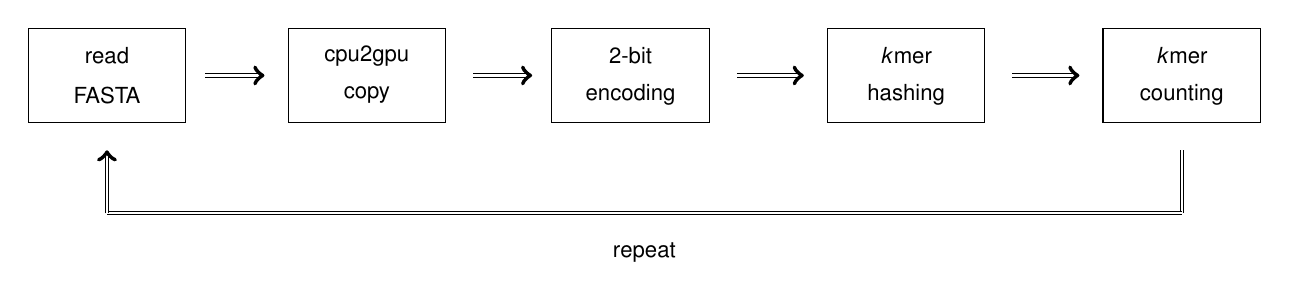
\begin{tikzpicture}
  % read fasta
  \node at(0,0)[draw,minimum width=2cm,minimum height=1.2cm](start){};
  \node at(0,.25)[]{\fontfamily{phv}\selectfont\smaller{read}};
  \node at(0,-.25)[]{\fontfamily{phv}\selectfont\smaller{FASTA}};
  \draw [double distance=.75pt,->](1.25,0) -- (2,0);
  % cpu2gpu copy
  \node at(3.3,0)[draw,minimum width=2cm,minimum height=1.2cm]{};
  \node at(3.3,.25)[]{\fontfamily{phv}\selectfont\smaller{cpu2gpu}};
  \node at(3.3,-.25)[]{\fontfamily{phv}\selectfont\smaller{copy}};
  \draw [double distance=.75pt,->](4.65,0) -- (5.4,0);
  % 2-bit encoding
  \node at(6.65,0)[draw,minimum width=2cm,minimum height=1.2cm]{};
  \node at(6.65,.25)[]{\fontfamily{phv}\selectfont\smaller{2-bit}};
  \node at(6.65,-.25)[]{\fontfamily{phv}\selectfont\smaller{encoding}};
  \draw [double distance=.75pt,->](8,0) -- (8.85,0);
  % kmer hashing
  \node at(10.15,0)[draw,minimum width=2cm,minimum height=1.2cm]{};
  \node at(10.15,.25)[]{\fontfamily{phv}\selectfont\smaller{\textit{k}mer}};
  \node at(10.15,-.25)[]{\fontfamily{phv}\selectfont\smaller{hashing}};
  \draw [double distance=.75pt,->](11.50,0) -- (12.35,0);
  % kmer counting
  \node at(13.65,0)[draw,minimum width=2cm,minimum height=1.2cm](end){};
  \node at(13.65,.25)[]{\fontfamily{phv}\selectfont\smaller{\textit{k}mer}};
  \node at(13.65,-.25)[]{\fontfamily{phv}\selectfont\smaller{counting}};
  % arrows
  \draw [double distance=.75pt](13.65,-.95) -- (13.65,-1.75);
  \draw [double distance=.75pt](13.65,-1.75) -- (0,-1.75);
  \draw [double distance=.75pt,->](0,-1.75) -- (0,-.95);
  \node at(6.825,-2.25)[]{\fontfamily{phv}\selectfont\smaller{repeat}};
\end{tikzpicture}
}
\caption{
  GKAGE's current \textit{k}mer counting pipeline performs several steps in a sequential fashion.
  While these steps are performed on many \textit{k}mers in parallel at once, each chunk (containing many \textit{k}mers) is processed sequentially. 
}
\label{discussion:parallelization_of_kmer_chunk_preparation:figures:pipeline}
\end{center}
\end{figure}

By utilizing CUDA streams we can parallelize the copying of data to the GPU and the processing of the previous chunk, creating a new and more efficient pipeline.

\begin{figure}[H]
\begin{center}
\scalebox{.9}{
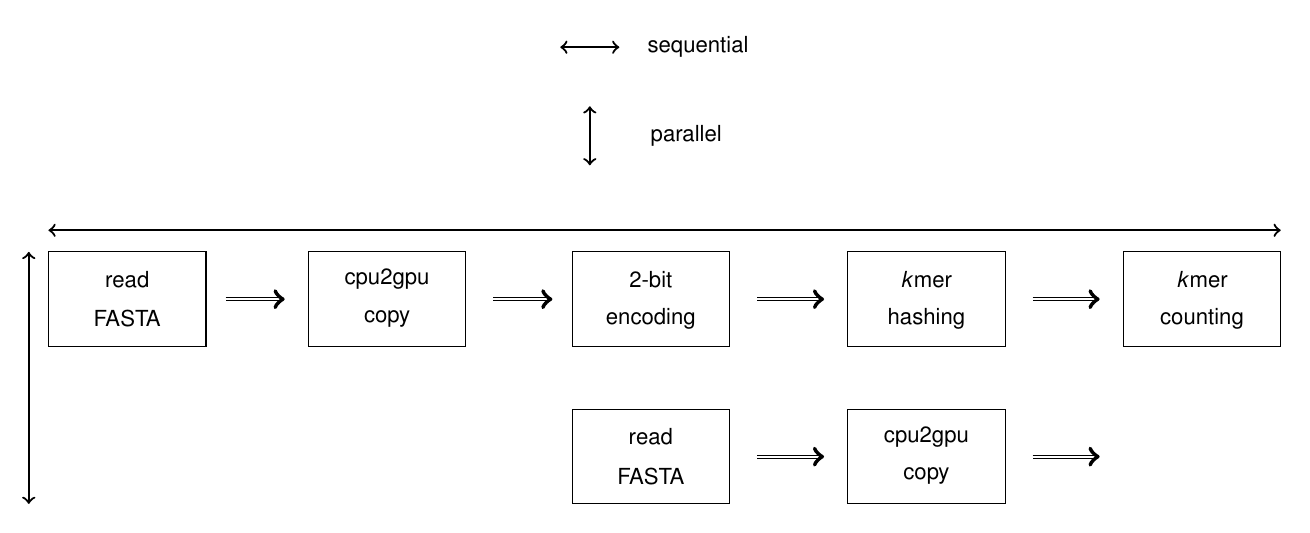
\begin{tikzpicture}
  % hints
  \draw [thick,<->](5.875,2.45) -- (5.875,1.7);
  \node at(7.1,2.075)[]{\fontfamily{phv}\selectfont\smaller{parallel}};
  \draw [thick,<->](5.5,3.2) -- (6.25,3.2);
  \node at(7.25,3.2)[]{\fontfamily{phv}\selectfont\smaller{sequential}};
  % large hints
  \draw [thick,<->](-1.25,.6) -- (-1.25,-2.6);
  \draw [thick,<->](-1,.875) -- (14.65,.875);
  % read fasta
  \node at(0,0)[draw,minimum width=2cm,minimum height=1.2cm](start){};
  \node at(0,.25)[]{\fontfamily{phv}\selectfont\smaller{read}};
  \node at(0,-.25)[]{\fontfamily{phv}\selectfont\smaller{FASTA}};
  \draw [double distance=.75pt,->](1.25,0) -- (2,0);
  % cpu2gpu copy
  \node at(3.3,0)[draw,minimum width=2cm,minimum height=1.2cm]{};
  \node at(3.3,.25)[]{\fontfamily{phv}\selectfont\smaller{cpu2gpu}};
  \node at(3.3,-.25)[]{\fontfamily{phv}\selectfont\smaller{copy}};
  \draw [double distance=.75pt,->](4.65,0) -- (5.4,0);
  % 2-bit encoding
  \node at(6.65,0)[draw,minimum width=2cm,minimum height=1.2cm]{};
  \node at(6.65,.25)[]{\fontfamily{phv}\selectfont\smaller{2-bit}};
  \node at(6.65,-.25)[]{\fontfamily{phv}\selectfont\smaller{encoding}};
  \draw [double distance=.75pt,->](8,0) -- (8.85,0);
  % kmer hashing
  \node at(10.15,0)[draw,minimum width=2cm,minimum height=1.2cm]{};
  \node at(10.15,.25)[]{\fontfamily{phv}\selectfont\smaller{\textit{k}mer}};
  \node at(10.15,-.25)[]{\fontfamily{phv}\selectfont\smaller{hashing}};
  \draw [double distance=.75pt,->](11.5,0) -- (12.35,0);
  % kmer counting
  \node at(13.65,0)[draw,minimum width=2cm,minimum height=1.2cm](end){};
  \node at(13.65,.25)[]{\fontfamily{phv}\selectfont\smaller{\textit{k}mer}};
  \node at(13.65,-.25)[]{\fontfamily{phv}\selectfont\smaller{counting}};
  % read fasta 2
  \node at(6.65,-2)[draw,minimum width=2cm,minimum height=1.2cm](start){};
  \node at(6.65,-1.75)[]{\fontfamily{phv}\selectfont\smaller{read}};
  \node at(6.65,-2.25)[]{\fontfamily{phv}\selectfont\smaller{FASTA}};
  \draw [double distance=.75pt,->](8,-2) -- (8.85,-2);
  % cpu2gpu copy 2
  \node at(10.15,-2)[draw,minimum width=2cm,minimum height=1.2cm]{};
  \node at(10.15,-1.75)[]{\fontfamily{phv}\selectfont\smaller{cpu2gpu}};
  \node at(10.15,-2.25)[]{\fontfamily{phv}\selectfont\smaller{copy}};
  \draw [double distance=.75pt,->](11.5,-2) -- (12.35,-2);
\end{tikzpicture}
}
\caption{
  An illustration of a more optimal \textit{k}mer counting pipeline.
  By utilizing CUDA's streams, we can parallelize copying of data to the GPU and actual GPU processing.
}
\label{discussion:parallelization_of_kmer_chunk_preparation:figures:parallel_pipeline}
\end{center}
\end{figure}



\newpage
\section{Conclusion} \label{conclusion}
In section \ref{introduction:thesis_goals}, we stated that one of the two goals of this thesis was to explore whether alignment-free genotyping could be sped up in any significant way by using the GPU.
To investigate this, we attempted to GPU accelerate an existing genotyper, KAGE, which recently showed that it was an order of magnitude faster than any other known genotyper \cite{kage}.
As a result of GPU accelerating components of KAGE, we presented GKAGE (GPU KAGE), a new GPU accelerated version of KAGE.
GKAGE achieves up to 5X speedup compared to KAGE on a high-end compute server, and more than 10X speedup on commercial hardware, all while using very little GPU memory - a scarce resource.
We believe that GKAGE is a useful contribution to the world of bioinformatics, considering the rate of which whole-genome sequencing is becoming more accessible and tools to analyze the generated sequence data is becoming increasingly necessary.

The second goal we presented in section \ref{introduction:thesis_goals}, was to investigate and experiment with different ways of GPU accelerating existing Python code that relies on array-programming libraries such as NumPy \cite{numpy}, and to reveal the advantages and drawbacks of such methods.
We achieved this by GPU accelerating different components of KAGE using a suite of different methods.
For each method, we discussed its advantages and drawbacks, where dimensions such as ease-of-use, seamless integration and performance were central.
We see the insights revealed by exploring these methods as showing that GPU acceleration is a feasible avenue to unlock performance enhancements in existing tools, particularly tools relying on large array-computations.
%As large array-computations are commonplace in computational biology, and as GPU acceleration libraries such as CuPy \cite{cupy} are making GPU acceleration more accessible even to programmers without much knowledge about GPUs, we believe that there could be an avalanche of existing methods and tools that could benefit from integrating such acceleration.
Large array-computations are commonplace in computational biology.
Additionally, Python GPU acceleration libraries such as CuPy \cite{cupy} are making GPU acceleration more accessible, even to programmers with limited knowledge of the GPU's programming model and hardware.
Given these factors, we believe that there could be an avalanche of existing methods and tools that could greatly benefit from integration such acceleration.


% bibliography
\newpage
\printbibliography

\end{document}
